%!TEX root=ClassNotes.tex

\section{Differentiation}
\begin{remark}
	We'll now exclusively work with {\it continuous} functions. As such, we can compute the various limits in this section without requiring any $\epsilon, \delta$ arguments. We'll get back to the $\epsilon, \delta$'s much later. For now, we'll repeated use the following identities,
	\begin{align*}
		\lim \limits_{x \rightarrow a} f(x) + g(x)     & = \lim \limits_{x \rightarrow a} f(x) + \lim \limits_{x \rightarrow a} g(x)                                                                   \\
		\lim \limits_{x \rightarrow a} f(x) \cdot g(x) & = \lim \limits_{x \rightarrow a} f(x) \cdot \lim \limits_{x \rightarrow a} g(x)                                                               \\
		\lim \limits_{x \rightarrow a} f(x) / g(x)     & = \lim \limits_{x \rightarrow a} f(x) / \lim \limits_{x \rightarrow a} g(x)     & \mbox{ assuming }\lim \limits_{x \rightarrow a} g(x) \neq 0
	\end{align*}
	wherever the appropriate limits exist.
\end{remark}

\subsection{Derivative}

The derivative of a function measures the {\it instantaneous rate of change} of the function. Several quantities in physics can be naturally expressed as derivatives, which was the original motivation for defining them.
\begin{center}
	\begin{tabular}{l|l}
		Function  & Derivative   \\ \hline
		Position  & Velocity     \\
		Velocity  & Acceleration \\
		Potential & Force
	\end{tabular}
\end{center}

\begin{definition}
	The {\bf derivative} of $f(x)$ with respect to $x$, at $x=a$, is defined to be the limit
	\begin{align}
		\label{eq:def_derivative}
		f'(a)
		 & :=
		\lim \limits_{h \rightarrow 0}
		\dfrac{f(a+h) - f(a)}{h}
	\end{align}
	If $f'(a)$ exists then we say that $f(x)$ is {\bf differentiable} at $a$.
\end{definition}
One can rewrite Equation \eqref{eq:def_derivative} as
\begin{align}
	\label{eq:def_derivative2}
	f'(a)
	 & =
	\lim \limits_{x \rightarrow a}
	\dfrac{f(x) - f(a)}{x - a}
\end{align}
by making the substitution $h = x - a$.

In this form, it is more explicit that derivative is computing the {\it instantaneous rate of change}, as the numerator $f(x) - f(a)$ is the change in $f$ and the denominator $x - a$ is the change in $x$, so their ratio is the rate of change of $f(x)$ with respect to $x$. Taking the limit $x \rightarrow a$ makes this rate of change {\it instantaneous}. When we want to make the ``free variable'' more explicit, we write the derivative as
\begin{align*}
	\left.\dfrac{df}{dx}\right|_{x = a}
\end{align*}
This notation becomes more relevant in multivariable calculus when there are multiple variables with respect to which one can differentiate the function.

\begin{exercise}
	\label{q:derivatives_1}
	Using the definition, compute the derivatives of the following functions.
	\begin{enumerate}
		\item $f(x) = c$, where $c$ is a real number.
		\item $f(x) = x$.
		\item $f(x) = x^2$.
	\end{enumerate}
\end{exercise}

\begin{exercise}
	Prove that if $f(x)$ is differentiable at $a$ then $f(x)$ is continuous at $x = a$.
\end{exercise}

\begin{theorem}
	\label{thm:derivative_rules}
	If $f$ and $g$ are differentiable at $a$ then\\
	\begin{align*}
		(f+g)'(a)                     & = f'(a) + g'(a)                                                                     \\\\
		(f\cdot g)'(a)                & = f'(a) \cdot g(a) + f(a) \cdot g'(a)                 &  & \mbox{\bf Product Rule}  \\\\
		\left(\dfrac{1}{g}\right)'(a) & = -\dfrac{g'(a)}{g(a)^2}                                                            \\\\
		\left(\dfrac{f}{g}\right)'(a) & = \dfrac{g(a) \cdot f'(a) - g'(a) \cdot f(a)}{g(a)^2} &  & \mbox{\bf Quotient Rule} \\\\
		(f\circ g)'(a)
		                              & = f'(g(a)) \cdot g'(a)                                &  & \mbox{\bf Chain Rule}    \\
	\end{align*}
	where we assume that $g(a) \neq 0$ wherever it is in the denominator.\\
\end{theorem}

\begin{exercise}
	Prove Theorem \ref{thm:derivative_rules}.

	The proof of the Product Rule requires a trick: add and subtract $f(a+h) g(a)$ to the numerator.

	For proving the Quotient Rule notice that $f/g = f \cdot (1/g)$.

	Feel free to read the proof of the Chain Rule from the book.
\end{exercise}

Because of these rules, once we know the derivatives of standard functions like trig functions, exponential functions etc., derivatives are fairly easy to compute. However, computing these standard derivatives is not easy using simply the definition (give it a try!).

Polynomials are the only functions whose derivatives we can compute right now. We'll get back to computing more complicated derivatives once we learn integration and the Fundamental Theorem of Calculus.


\begin{exercise} In this exercise we'll (almost) prove that
	\begin{align}
		\label{eq:polynomial_derivative}
		(x^n)' = n x^{n -1}
	\end{align}
	where $n$ is any real number.

	Note that Exercise \ref{q:derivatives_1} proves this for the cases $n = 0, 1, 2$.
	\begin{enumerate}
		\item Use the identity $(x^{n}) \cdot x = x^{n + 1}$ to prove \eqref{eq:polynomial_derivative} for all positive integers.\footnote{{\bf Optional:} Read about {\bf Mathematical Induction} and use it to write a rigorous proof of this statement.}
		\item Use the identity $\frac{1}{x^m} = x^{-m}$ to prove \eqref{eq:polynomial_derivative} for all negative integers.
		\item Use the $\left( x^{\frac{p}{q}}\right)^q = x^p$ to prove \eqref{eq:polynomial_derivative} for all rational numbers.
	\end{enumerate}
	This proves \eqref{eq:polynomial_derivative} for all rational numbers. We do not yet know enough to extend this proof to irrationals.
	\begin{enumerate}[resume]
		\item Can you think of a way to prove \eqref{eq:polynomial_derivative} for all real numbers? What fact {\it should} be true for your proof to work?
	\end{enumerate}
\end{exercise}


\subsection{Inverse Functions}
We say that functions $f$ and $g$ are {\bf inverses} of each other if the following identities hold:
\begin{align*}
	f (g(x)) & = x \\
	g(f(x))  & = x
\end{align*}

\begin{exercise}
	Verify that if $f$ and $g$ are inverses of each other and $f(x) = y$ then $x = g(y)$. (Hence the name inverse.)
\end{exercise}
This exercise is saying that to find the inverse of $f(x)$ we simply solve $f(x) = y$ for $x$ in terms of $y$, which then gives us $g$.


\begin{exercise}$ $
	\begin{enumerate}
		\item Verify that $f(x) = 2x + 1$ and $g(x) = (x-1)/2$ are inverses of each other. Draw their graphs.
		\item Verify that $f(x) = x^2$ and $g(x) = \sqrt{x}$ are inverses of each other. Draw their graphs.
		\item Verify that $f(x) = e^x$ and $g(x) = \ln x$ are inverses of each other.
		      Draw their graphs.
		\item What relation do you see between the graphs of inverses?
		\item What are the domains of these functions i.e. what is the set of real numbers where the these functions are defined? Why do you think some of the inverses are not defined everywhere?
	\end{enumerate}
\end{exercise}

The inverses of $\sin x$ and $ \cos x$ are denoted $\sin^{-1} (x)$ and $\cos^{-1} (x)$, respectively. More generally, the inverse of a function $f(x)$ is denoted by $f^{-1}(x)$ (which is different from $(f(x))^{-1}$). Note that if $f = g^{-1}(x)$ then $g = f^{-1}(x)$.

\begin{exercise}
	Using the Chain Rule show that
	\begin{align*}
		\left(f^{-1}(a)\right)'= \dfrac{1}{f'(f^{-1}(a))}
	\end{align*}
	Verify this explicitly for $f(x) = 2x+1$ and for $f(x) = x^2$.
\end{exercise}
We'll interpret this geometrically in the next section. We'll later on see that the derivatives of $\sin^{-1}(x)$ and $\ln x$ can expressed in terms of polynomials and radicals. This fact along with the above formula will then allow us to compute the derivatives of $\sin x$ and $e^x$.








\subsection{Mean Value Theorems}
Derivatives have several physical and geometric interpretations which make then widely applicable in all branches of science. We'll see a few of these interpretations in the next few sections.

In this section, we'll prove the analogues of Intermediate Value Theorem for differentiable functions.

\begin{definition}
	A number $c$ is an {\bf absolute maximum} of a function $f$ in the interval $[a,b]$ if $f(c) \ge f(x)$ for all $x \in [a,b]$.
\end{definition}
To prove the Mean Value Theorems we'll need the following {\bf Extreme Value Theorem}. We'll assume it without proof. As for the IVT, the proof of the Extreme Value Theorem fundamentally uses the Completeness of the Real Numbers.

\begin{theorem}[Extreme Value Theorem]
	\label{thm:extreme_value_theorem}
	For every continuous function $f$ and every closed interval $[a,b]$, there exists a real number $c \in [a,b]$ such that $c$ is the absolute maximum of $f$ on $[a,b]$.
\end{theorem}

\begin{remark}
	This theorem is false if we use open intervals. For example, $f(x) = 1/x$ has no absolute maximum on the interval $(0,1)$ even though it is continuous on it.
\end{remark}

\begin{exercise}
	Define an absolute minimum and state the corresponding Extreme Value Theorem.
\end{exercise}

% \begin{exercise}
% 	Let $f$ be a differentiable (and hence also continuous) function. On an interval $[a,b]$, by the Extremal Value Theorem, $f$ has an absolute maxima. Let $c$ be the absolute maximum. Assume that $a < c <b$.
% 	\begin{enumerate}
% 		\item Argue that the function $g(x) = \dfrac{f(x) - f(c)}{x - c}$ is $\ge 0$ for $ a < x < c$ and is $\le 0$ for $c < x < b$.
% 		\item Argue that $\lim \limits_{x \rightarrow c^-}g(x) \ge 0$ and $\lim \limits_{x \rightarrow c^+}g(x) \le 0$.
% 		\item Conclude that $f'(c) = 0$.
% 	\end{enumerate}
% \end{exercise}
%
% Thus we've proven the following theorem
% \begin{theorem}
% 	\label{thm:max_derivative}
% 	Let $f$ be a differentiable function. If $c$ is an absolute maximum for $f$ on the interval $[a,b]$ with $a < c < b$ then $f'(c) = 0$. Similar statement is true for an absolute minimum.
% \end{theorem}

Note that by our definitions an {\it absolute} max/min $c$ of $f$ over $[a,b]$ is also a {\it local} max/min if $a < c < b$. We've already shown that the derivative vanishes at a local max/min, so we have
\begin{theorem}
	\label{thm:max_derivative}
	Let $f$ be a differentiable function. If $c$ is an absolute max/min for $f$ on the interval $[a,b]$ with $a < c < b$ then $f'(c) = 0$.
\end{theorem}

This is all we'll be needing to prove the various Mean Value Theorems.

\begin{theorem}[Rolle's Theorem]
	Let $f$ be a differentiable function. For an interval $[a,b]$, if
	\begin{align*}
		f(a) = f(b)
	\end{align*}
	then there exists a real number $c \in (a,b)$ such that
	\begin{align*}
		f'(c) = 0
	\end{align*}
	\begin{figure}[H]
		\centering
		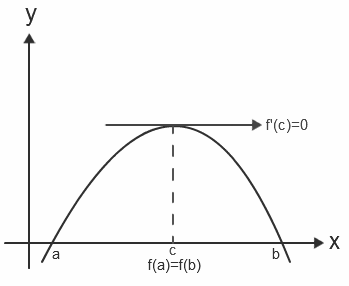
\includegraphics[width=0.6\textwidth]{RollesTheorem.png}
	\end{figure}
\end{theorem}
\begin{proof}[Proof of Rolle's Theorem]
	This theorem almost immediately follows from Theorem \ref{thm:extreme_value_theorem} and Theorem \ref{thm:max_derivative}. The only issue is that for Theorem \ref{thm:max_derivative} we need $a < c < b$ but the Extreme Value Theorem only guarantees $a \le c \le b$. So we need a small argument to fill this gap.

	By the Extremal Value Theorem, $f$ has an absolute maximum $c_{\max}$ and an absolute minimum $c_{\min}$ on the interval $[a,b]$.

	\begin{exercise}$ $
		\begin{enumerate}
			\item Argue that if $f(c_{\max}) = f(c_{\min})$ then $f$ is a constant function on $[a,b]$.
		\end{enumerate}
		We've already shown that for a constant function, $f'(x)$ equals 0, hence for every $c \in (a,b)$, $f'(c) = 0$ and we're done.

		So now we'll assume that $f(c_{\max}) \neq f(c_{\min})$.

		\begin{enumerate}[resume]
			\item 		Argue that in this case either $a < c_{\max} < b$ or $a < c_{\min}< b$ (possibly both).
			\item 		Finish the proof of Rolle's Theorem.
		\end{enumerate}
	\end{exercise}
\end{proof}

\begin{theorem}[Mean Value Theorem]
	Let $f$ be a differentiable function. For any interval $[a,b]$ there exists a real number $c \in (a,b)$ such that
	\begin{align*}
		f'(c) = \dfrac{f(b) - f(a)}{b - a}
	\end{align*}
	\begin{figure}[H]
		\centering
		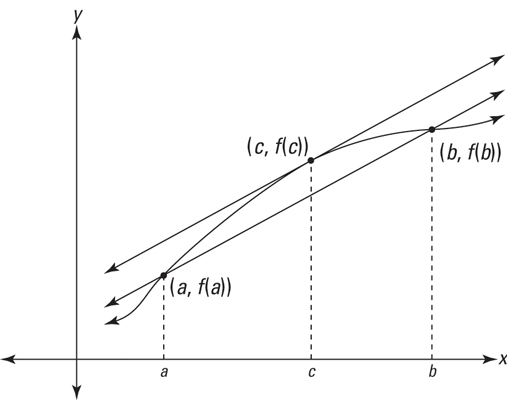
\includegraphics[width=0.6\textwidth]{MeanValueTheorem.jpg}
	\end{figure}
\end{theorem}
\begin{proof}[Proof of Mean Value Theorem]
	Mean Value Theorem follows from the Rolle's theorem by an algebraic trick.
	We'll construct a new function $g(x)$ that satisfies the hypotheses of Rolle's theorem.
	\begin{exercise}$ $
		\begin{enumerate}
			\item Find a real number $r$ such that $f(a) - r a = f(b) - r b$.
		\end{enumerate}
		For this value of $r$ define
		\begin{align*}
			g(x) = f(x) - r x
		\end{align*}
		By construction, $g$ is differentiable and satisfies $g(a) = g(b)$ and hence satisfies the hypotheses for Rolle's theorem. So, there exists some real number $ a < c < b$ such that
		\begin{align*}
			g'(c) = 0
		\end{align*}
		\begin{enumerate}[resume]
			\item Show that for this $c$, $f'(c) = \dfrac{f(b) - f(a)}{b - a}$, thereby completing the proof of Mean Value Theorem.
		\end{enumerate}
	\end{exercise}
\end{proof}

We'll see later on that the Mean Value Theorem is a key ingredient in the proof of Taylor series approximation. In fact, Taylor series approximations can be thought of as a generalization of MVT for higher order derivatives.




\subsection{L'Hopital's Rule}
We'll now (almost) provide a proof of L'Hopital's Rule using a stronger version of the Mean Value Theorem.
\begin{theorem}[Easy L'Hopital's Rule]
	Let $f$, $g$ be differentiable functions. Assume that
	\begin{align*}
		f(a) = 0 = g(a) \mbox{ \quad and \quad } g'(a) \neq 0,
	\end{align*}
	where $a$ is a real number. Then
	\begin{align*}
		\lim \limits_{x \rightarrow a} \dfrac{f(x)}{g(x)} = \dfrac{f'(a)}{g'(a)}
	\end{align*}
\end{theorem}
\begin{exercise}
	Notice that $\dfrac{f(x)}{g(x)} = \dfrac{f(x) - f(a)}{g(x) - g(a)}$. Use this to prove the easy version of L'Hopital's Rule. \hint{Divide the numerator and denominator by $x - a$ and take $\lim \limits_{x \rightarrow a}$.}
\end{exercise}

\begin{theorem}[Strong Mean Value Theorem]
	Let $f$, $g$ be differentiable functions. Assume that $g(a) \neq g(b)$ for some real numbers $a$ and $b$. Then there exists a real number $c \in (a,b)$ such that
	\begin{align*}
		\dfrac{f'(c)}{g'(c)} = \dfrac{f(b) - f(a)}{g(b) - g(a)}
	\end{align*}
\end{theorem}
\begin{proof}[Proof of Strong Mean Value Theorem]
	The Strong Mean Value Theorem follows from the Rolle's theorem by the same algebraic trick. We'll construct a new function $h(x)$ that satisfies the hypotheses of Rolle's theorem.
	\begin{exercise}$ $
		\begin{enumerate}
			\item Find a real number $r$ such that $f(a) - r g(a) = f(b) - r g(b)$.
		\end{enumerate}
		For this value of $r$ define
		\begin{align*}
			h(x) = f(x) - r g(x)
		\end{align*}
		By construction, $h$ is differentiable and satisfies $h(a) = h(b)$ and hence satisfies the hypotheses for Rolle's theorem. So, there exists some real number $ a < c < b$ such that
		\begin{align*}
			h'(c) = 0
		\end{align*}
		\begin{enumerate}[resume]
			\item Show that for this $c$, $\dfrac{f'(c)}{g'(c)} = \dfrac{f(b) - f(a)}{g(b) - g(a)}$, thereby completing the proof of the Strong Mean Value Theorem.
		\end{enumerate}
	\end{exercise}
\end{proof}

\begin{exercise}
	Explain how the Mean Value Theorem is a special case of the Strong Mean Value Theorem and how the Rolle's theorem is a special case of the Mean Value Theorem.
\end{exercise}
\begin{theorem}[L'Hopital's Rule]
	Let $f$, $g$ be differentiable functions. Assume that
	\begin{align*}
		f(a) = 0 = g(a)
	\end{align*}
	where $a$ is a real number. Then
	\begin{align*}
		\lim \limits_{x \rightarrow a} \dfrac{f(x)}{g(x)} = \lim \limits_{x \rightarrow a} \dfrac{f'(x)}{g'(x)}
	\end{align*}
\end{theorem}

\begin{proof}[Idea of the proof]
	For any $b$, by the Strong Mean Value Theorem, there exists a $c \in (a,b)$ such that
	\begin{align*}
		\dfrac{f'(c)}{g'(c)}          & = \dfrac{f(b) - f(a)}{g(b) - g(a)}                                \\
		\implies \dfrac{f'(c)}{g'(c)} & = \dfrac{f(b)}{g(b)}               & (\mbox{as } f(a) = 0 = g(a))
	\end{align*}
	As $c$ has to lie between $a$ and $b$, when we take the limit $b \rightarrow a$ we must also have $c \rightarrow a$. Taking limits of both sides we get the required result.
	\begin{align*}
		\lim \limits_{c \rightarrow a} \dfrac{f'(c)}{g'(c)} = \lim \limits_{b \rightarrow a}  \dfrac{f(b)}{g(b)}
	\end{align*}
\end{proof}

\begin{remark}
	The last argument in the above proof is not rigorous. While the idea is correct, to make it rigorous we need generalized notions of limits called {\bf limit superior} ($\lim \sup$) and {\bf limit inferior} ($\lim \inf$). This is unfortunately beyond the scope of this class.
\end{remark}

There are many more variants of L'Hopital's Rule: for one-sided limits, for $a = \infty$, for $ \lim \limits_{x \rightarrow a} f(a)= \infty =\lim \limits_{x \rightarrow a} g(a) $ etc. They can all be proven using similar techniques.










\subsection{First Derivative Test}
In this section, we'll prove the First Derivative Test for differentiable functions.

\begin{definition}
	We say that a function $f$ is {\bf increasing} on an interval $[a,b]$, if for all $x$, $y$ in $[a,b]$ if $x < y$ then $f(x) \le f(y)$.
		We say that $f$ is {\bf strictly increasing} on $[a,b]$, if for all $x$, $y$ in $[a,b]$ if $x < y$ then $f(x) < f(y)$.
\end{definition}
\begin{exercise}
	Come up with a definition for when a function is {\bf decreasing}, {\bf strictly decreasing} on an interval.
\end{exercise}
\begin{exercise}
	Find the interval(s) on which the function $x^2$ is increasing/decreasing? What about the function $x^3$?
\end{exercise}

For differentiable functions, we can determine if a function is increasing or decreasing by calculating it's first derivative.
\begin{exercise}$ $
	\label{q:increasing_decreasing_derivative}
	\begin{enumerate}
		\item {\bf Optional:} Let $g(x)$ be a function such that $\lim \limits_{x\rightarrow c} g(x)$ exists for some real number $c$ in the interval $(a,b)$. Prove that if $g(x) \ge 0$ for all $x$ in $[a,b]$, then $\lim \limits_{x\rightarrow c} g(x)$ is also $\ge 0$.\hint{Proof by Contradiction.}\\ {\it (You can assume this part to be true if you choose not to prove it.)}
		\item Let $f(x)$ be an increasing function on $[a,b]$ and let $c \in (a,b)$. Prove that $g(x) \ge 0$ on the interval $[a,b]$ where $g(x)$ is the function
		      \begin{align*}
			      g(x) = \dfrac{f(x) - f(c)}{x - c}
		      \end{align*}
		\item Let $f(x)$ be a differentiable function that is increasing on the interval $[a,b]$. Prove that all $c \in (a,b)$, $f'(c) \ge 0$. Similarly, for decreasing functions.
	\end{enumerate}
\end{exercise}
Note that this agrees with the interpretation of a derivative as the {\it instantaneous} rate of change of a function: an increasing function should have a positive {instantaneous} rate of change and a decreasing function should have a negative {instantaneous} rate of change. The converse of the above statement is almost true, but for this we need an extra assumption on $f$ and the proof is a bit more intricate.

\begin{prop}
	\label{thm:increasing_positive_derivative}
	If $f'(x) > 0$ for all $c \in (a,b)$ then $f$ is strictly increasing on $(a,b)$. Similarly, for $f'(c) < 0$.
\end{prop}

\begin{exercise}
	Let $f'(x) > 0$ for all $c \in (a,b)$. Prove by Contradiction, that for all $x$, $y \in (a,b)$, if $x < y$ then $f(x) < f(y)$.\hint{Use the Mean Value Theorem.}
\end{exercise}

\begin{exercise}
	Use the above Proposition to find the range in which the function $x^n$ is increasing/decreasing, where $n$ is a positive integer.
\end{exercise}

\begin{definition}A real number $c$ is said to be a {\bf local maximum} of a function $f$ if there is some interval $(a,b)$ containing $c$ such that if $a < x < b$ then $f(c) \ge f(x)$.
\end{definition}
\begin{exercise}
	Come up with a definition for {\bf local minimum}.
\end{exercise}
\begin{exercise} Assume that the function $f(x)$ is differentiable and it's derivative $f'(x)$ is continuous. Using Proposition \ref{thm:increasing_positive_derivative} prove that if $c$ is a local maximum of $f(x)$ then $f'(c) = 0$.\hint{Proof by Contradiction.} Similarly for a local minimum.
\end{exercise}
\begin{remark}
	We need $f'(x)$ to be continuous to ensure that if $f'(c) > 0$ then $f'(x) > 0$ for every $ x \in (a,b)$, where $(a,b)$ is some interval containing $c$.
\end{remark}



Combining everything in this section we have proven the following Theorem, also called the {\bf First Derivative Test}.
\begin{theorem}[First Derivative Test]
	Let $f(x)$ be a differentiable function whose derivative $f'(x)$ is a continuous function.

	For a real number $c$,
	\begin{align*}
		f	\mbox{ has a local max/min at } c & \implies f'(c) = 0   \\
		f \mbox{ is increasing near } c    & \implies f'(c) \ge 0 \\
		f \mbox{ is decreasing near } c    & \implies f'(c) \le 0
	\end{align*}
	Conversely,
	\begin{align*}
		f'(c) > 0 & \implies f \mbox{ is increasing near } c \\
		f'(c) < 0 & \implies f \mbox{ is decreasing near } c
	\end{align*}
	where by ``near $c$'' means for some interval $(a,b)$ containing $c$.
\end{theorem}

A real number $c$ satisfying $f'(c) = 0$ is called a {\bf critical point} of $f$. The First Derivative Test says that a local max/min has to be a critical point, but it does not say that a critical point has to be a local max/min. A standard example of this failure is $c=0$ for the function $f(x) = x^3$.
\begin{align*}
	\mbox{Local min/max}  & \Rightarrow \mbox{Critical point}    \\
	\mbox{Critical point} & \not\Rightarrow \mbox{Local min/max}
\end{align*}
There are ways to fix this using higher derivatives. We'll do this later using Taylor Series approximations.



\subsubsection*{Optional Problems}
There are multiple ways of proving Proposition \ref{thm:increasing_positive_derivative}. However, all the methods require some additional techniques which we have not yet developed.

\begin{exercise}
	Try to write down a rigorous proof of Proposition \ref{thm:increasing_positive_derivative}. What statement {\it should} be true for your proof to work?
\end{exercise}









\subsection{Convexity and Concavity}
The second derivative of a function $f(x)$ is defined as
\begin{align*}
	f''(x) = \left(f'(x)\right)'
\end{align*}
If the second derivative exists then we say that a function is {\bf twice differentiable}.
More generally, the $n^{th}$ derivative $f^{(n)}(x)$ is defined as
\begin{align*}
	f^{(n)}(x) = \left(f^{(n-1)}(x)\right)'
\end{align*} If all derivatives exist then we say that the function is {\bf smooth} or {\bf infinitely differentiable}. The standard functions like polynomials, trig functions, exponentials, and logarithms are all smooth wherever they're defined.\\

If a function $f$ is twice differentiable, then the second derivative of $f$ measures it's convexity/concavity.
\begin{definition}
	A function $f$ is said to be {\bf convex} (or {\bf concave upwards}) on an interval, if for every real numbers $a$, $b$ in the interval, the graph of $f(x)$ lies below the line joining $(a,f(a))$ to $(b,f(b))$.
	\begin{figure}[H]
		\centering
		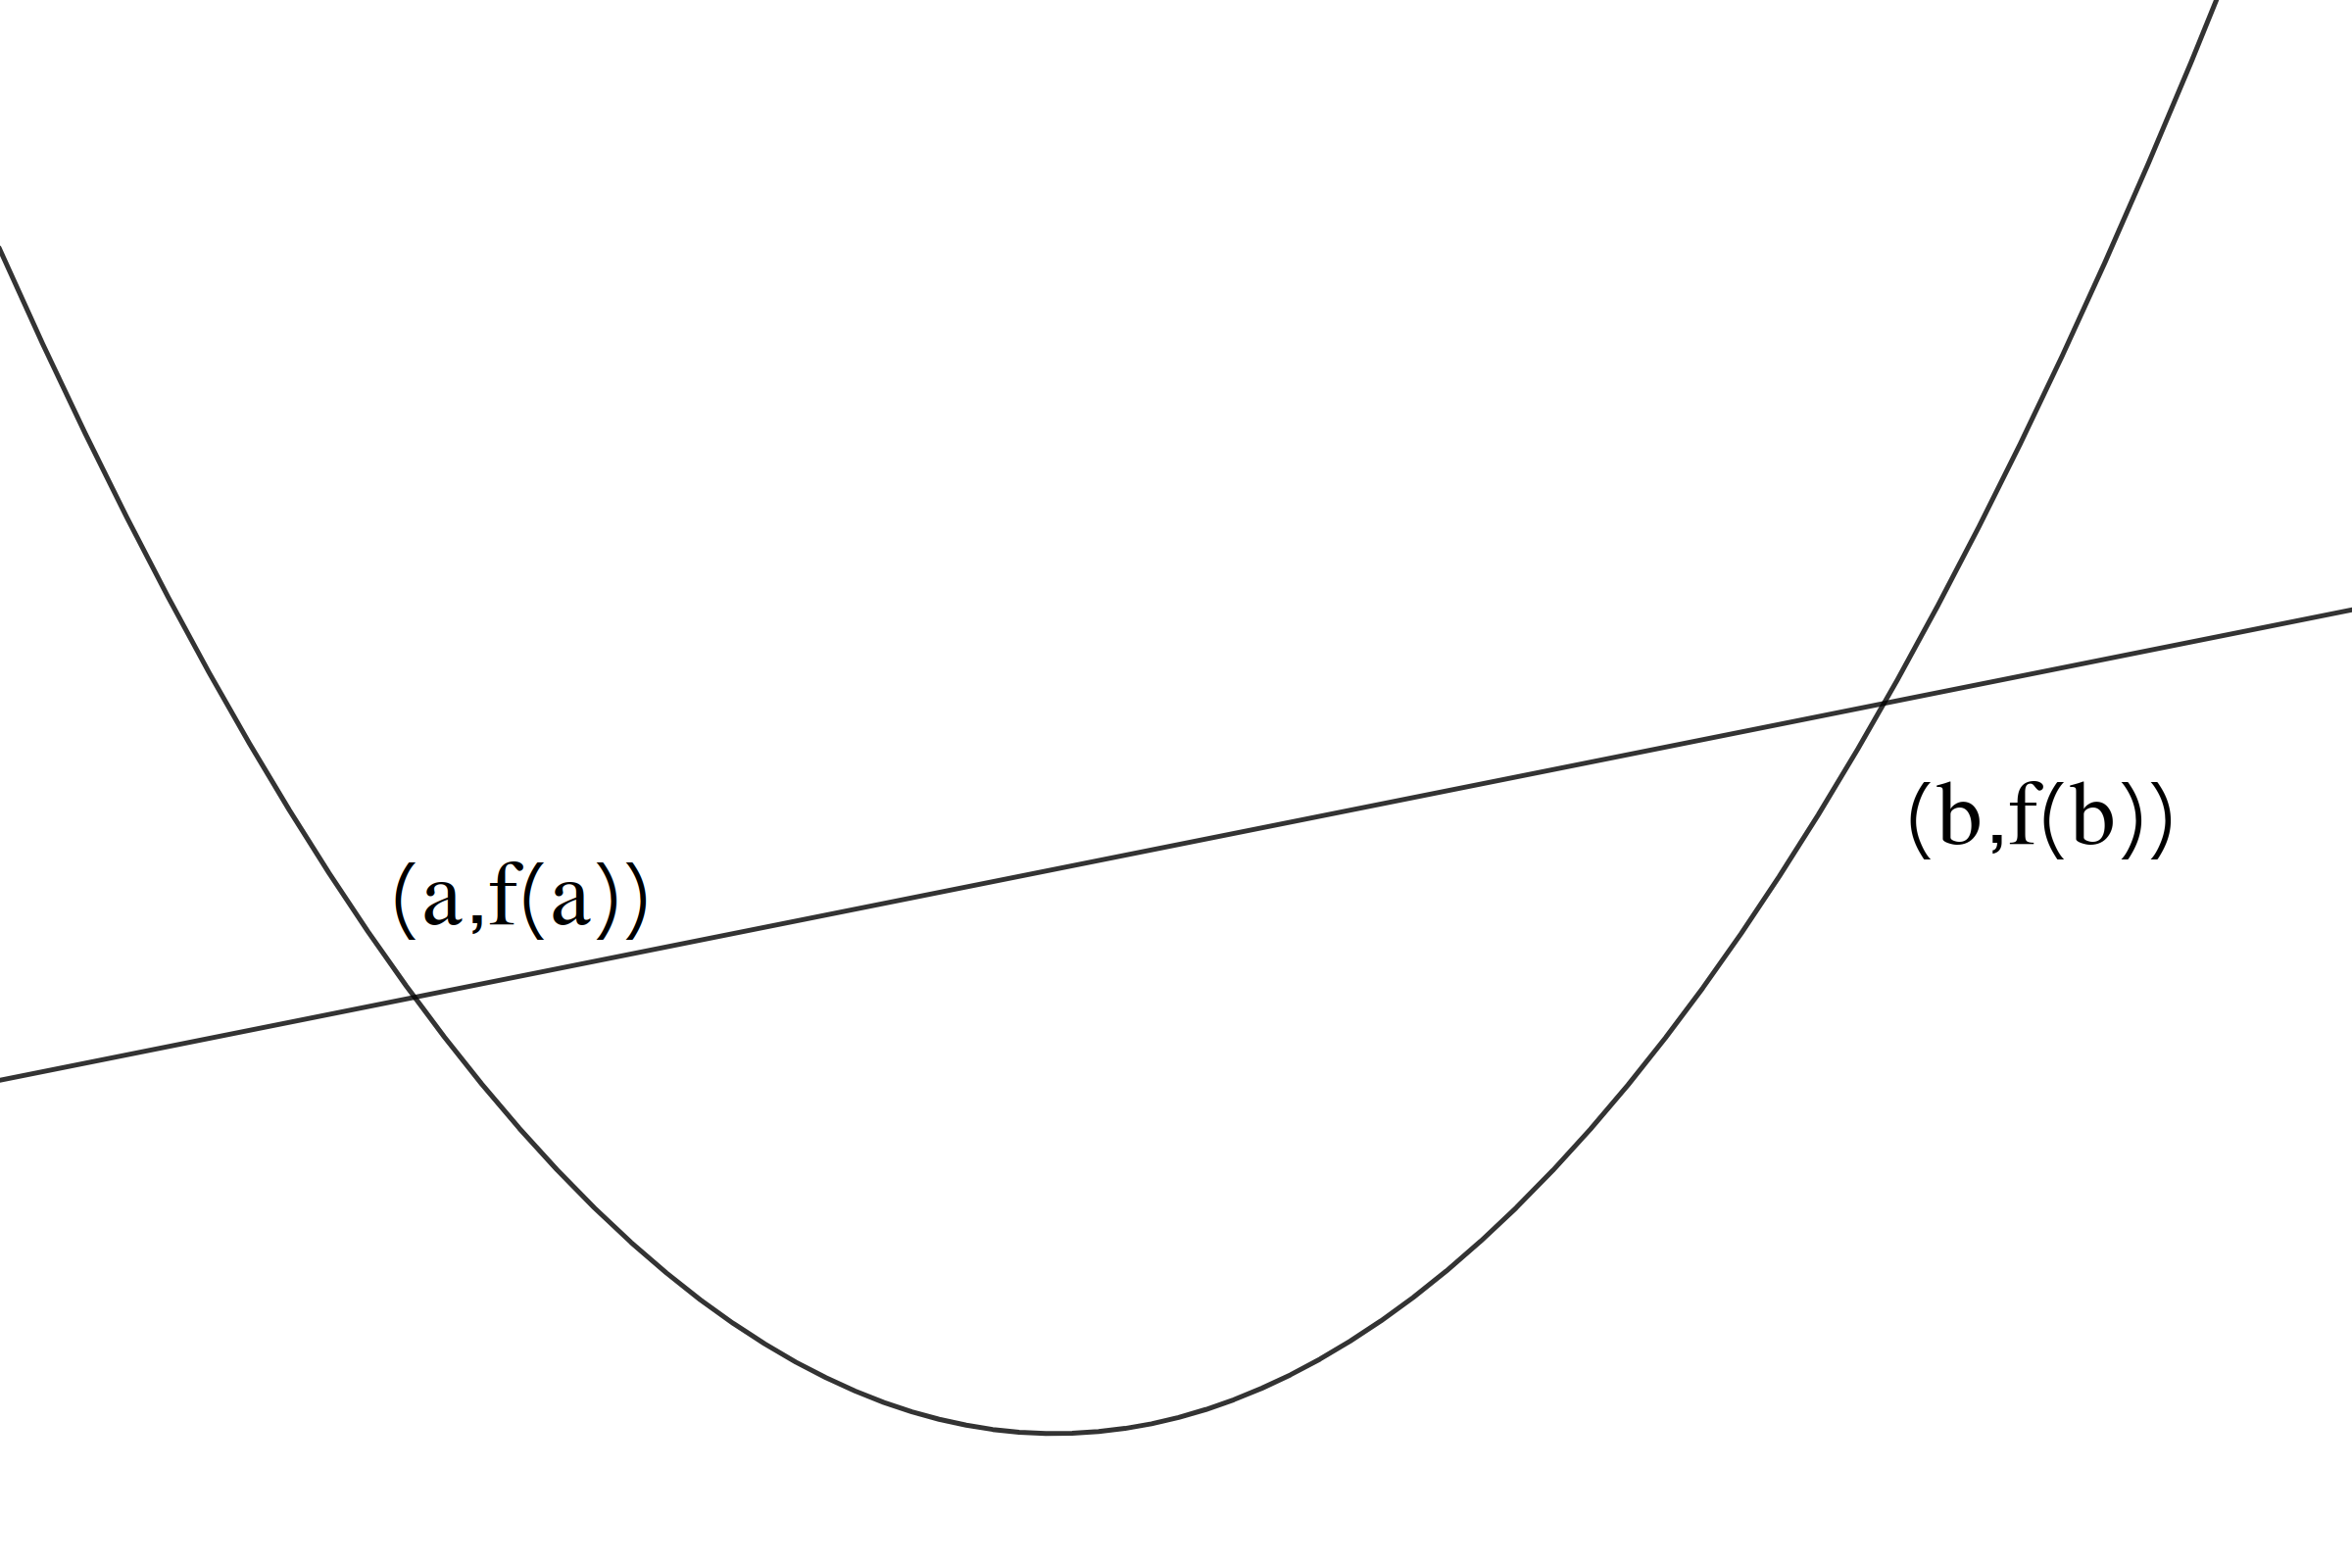
\includegraphics[width=0.6\textwidth]{ConvexFunction.png}
	\end{figure}
\end{definition}
Convex functions play an important role in many areas of mathematics, especially in the study of optimization problems.\\

The following theorem establishes the connection between convexity and the second derivative.
\begin{theorem}
	\label{thm:convex_functions}
	Let $f$ be a twice differential function.

	If $f$ is convex on an interval then $f''(x) \ge 0$ on that interval. Conversely, if for every real number $x$ in some interval, $f''(x) > 0$, then $f$ is convex on that interval.
\end{theorem}

\begin{remark}
	To avoid clutter, we'll often drop the terms {\it on an interval, in some interval} etc. in the following proof. Just keep in mind that there is an ambient interval and all our variables belong to that interval.
\end{remark}

\noindent \begin{tabular}{|p{\textwidth}|}
  \hline \\{\it Once you have solved all the exercises below, submit your final solutions as one single logically coherent proof. Also include all the text that is in between the exercises, so that you yourself see how all the pieces fit together. As before, this is to practice writing complex proofs.}\\\\
  \hline
\end{tabular}

\begin{proof}
	Let $f$ be a twice differential function.
	\begin{exercise}
		For real numbers $a$, $b$ denote by $m_{a,b}$ the slope of the line joining the points $(a,f(a))$ and $(b,f(b))$.
		Find a formula for $m_{a,b}$.
	\end{exercise}

	\noindent We'll first prove the forward direction.\\
	\noindent {\bf Claim:} {\it 	If $f$ is convex on an interval then $f''(x) \ge 0$ on that interval.}

	We'll prove that $f'(x)$ is an increasing function which will then imply that $f''(x) \ge 0$ (as the derivative of an increasing function is $\ge 0$).\\

	Let $f$ be a convex function. Let $a < b$ be two real numbers.
	\begin{exercise}
		Let $a < x < y$ be real numbers.
		\begin{enumerate}
			\item {\it Geometrically} argue that $m_{a,x} < m_{a,y}$.
			\begin{figure}[H]
				\centering
				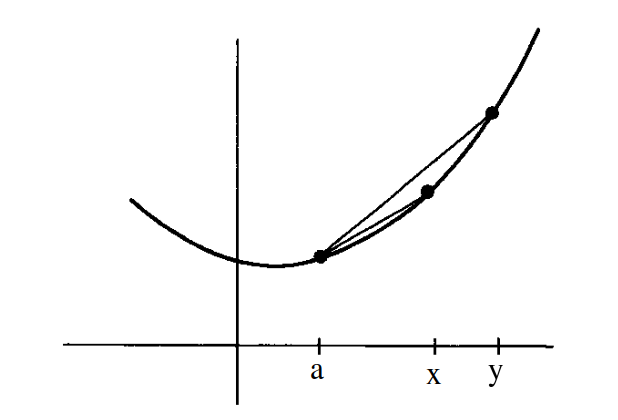
\includegraphics[width=0.6\textwidth]{ConvexFunctionProof1.png}
			\end{figure}
			\item Using the formula for $m_{a,x}$, $m_{a,y}$ and the above inequality argue that $$f'(a) \le m_{a,y}$$ for real numbers $a < y$.
		\end{enumerate}
	\end{exercise}

	\begin{exercise}
		Let $x < y < b$ be real numbers.
		\begin{enumerate}
			\item {\it Geometrically} argue that $m_{x,b} < m_{y,b}$.
			\item Using the formula for $m_{y,b}$, $m_{x,b}$ and the above inequality argue that $$m_{x,b} \le f'(b) $$ for real numbers $x < b$.
		\end{enumerate}
	\end{exercise}

	\begin{exercise}
		Combine the results from the previous two exercises to conclude that $f'(a) \le f'(b)$.
	\end{exercise}
	Hence $f'(x)$ is an increasing function and hence $f''(x) \ge 0$.\\

	\noindent We'll next prove the other direction. \\
	\noindent {\bf Claim:} {\it If for every real number $x$ in some interval, $f''(x) > 0$, then $f$ is convex on that interval.}

	We'll prove this by {\it contradiction}. Let $f$ be a function such that $f''(x) > 0$ on some interval. This implies that $f'(x)$ is an increasing function on that interval. This is the statement that we'll contradict.\\

	Assume on the contrary that $f$ is not convex. This means that for some real numbers $a < b$, there exists a number $c$ with $a < c < b$ such that the point $(c,f(c))$ lies above the line joining $(a,f(a))$ and $(b,f(b))$.

	\begin{exercise}
		Draw a picture.
	\end{exercise}
	Applying the Mean Value Theorem to the intervals $[a,c]$ and $[c,b]$ gives us real numbers $d_1 \in (a,c)$ and $d_2 \in (c,b)$ such that
	\begin{align*}
		f'(d_1) = m_{a,c} \mbox{ and } f'(d_2) = m_{c,b}
	\end{align*}

	\begin{exercise} $ $
		\begin{enumerate}
			\item Draw a picture.
			\item {\it Geometrically} argue that $f'(d_1) > f'(d_2)$.
			\item Why is this a contradiction?
		\end{enumerate}
	This completes a proof of the other direction, and hence of the main theorem.
	\end{exercise}
\end{proof}

\subsubsection{Second Derivative Test}
Let $f(x)$ be a twice differentiable function. If a real number $c$ is a local minimum of $f$ then $f$ is convex on some interval containing $c$. A similar statement is true when $c$ is a local maximum. Combining this observation with the previous Theorem and the First Derivative Test, we get the {\bf Second Derivative Test}.

\begin{theorem}[Second Derivative Test]
	Let $f(x)$ be a twice differentiable function whose second derivative $f''(x)$ is a continuous function.
	\begin{align*}
		f	\mbox{ has a local min at } c &\implies f'(c) = 0 \mbox{ and } f''(c) \ge 0 \\
			f	\mbox{ has a local max at } c &\implies f'(c) = 0 \mbox{ and } f''(c) \le 0
	\end{align*}
	Conversely,
	\begin{align*}
		f'(c) = 0 \mbox{ and } f''(c) > 0 & \implies f	\mbox{ has a local min at } c  \\
		f'(c) = 0 \mbox{ and } f''(c) < 0 & \implies f	\mbox{ has a local max at } c
	\end{align*}
\end{theorem}
We need continuity of $f''(x)$ so that $f''(c) > 0$ implies $f''(x)>0$ on some interval containing $c$.


\subsubsection*{Optional Problems}
\begin{exercise}$ $
	\begin{enumerate}
		\item Find an example of a function which is convex but $f''(x)$ is not always $> 0$.
		\item Why does the proof of Theorem \ref{thm:convex_functions} only proves  that {\it if $f$ is convex then $f''(x) \ge 0$} (instead of $f''(x) > 0$)?
	\end{enumerate}
\end{exercise}

\begin{exercise}
	Several times in this section we used {\it geometric} arguments. This is less preferable than algebraic arguments as geometric arguments are not rigorous and hence susceptible to being incorrect.
	\begin{enumerate}
		\item Convert the definition of a convex function into an algebraic equation involving inequalities.
		\item Use this equation to rigorously prove that, say, $m_{a,x} < m_{a,y}$ if $a < x < y$.
	\end{enumerate}
\end{exercise}

\begin{exercise}
	Let $f$ be a convex function on an interval containing the real numbers $a$, $b$. Show that for all $ t \in [0,1]$,
	\begin{align*}
		f(t a + (1-t) b) \le t f(a) + (1- t) f(b)
	\end{align*}
	This inequality is called {\bf Jensen's inequality} for convex functions.
\end{exercise}
